\chapter{Introduction}\label{ch:intro}

The following Master's thesis is divided into five chapters. In the first chapter, we will introduce the concept of criticality in complex systems, both living and non-living.  
We will also make a brief summary of stochastic processes and their relation to point processes and Hawkes processes, which are the main focus of this work.
After that, we will present the objectives of this work. In the third chapter, we will present the methodology used in this work, including the simulation of Hawkes processes, 
and the methodology for its analysis. In the second last chapter, we will present the results of the simulations, including the phase diagram of the process, the 
susceptibility analysis, and the avalanche analysis and we will discuss them. Finally, in the fifth chapter, we will present the conclusions of this work and the future lines of research.

\section{Criticality and its presence in living systems}

Criticality is one of the key concepts around complex systems because it is believed that they may benefit from by working in a critical state or near it. It has been demonstrated that
these states provide the system with desirable properties such as robustness, adaptability, information processing, and a wider dynamic range thanks to the scale invariance associated with the
critical states \cite{munoz2018colloquium}. This scale invariance can be described through a a specific probability distribution, named Pareto or power-law distribution like $P(t) = Ct^{-\gamma}$.
Where $\gamma\in\Re^+$ and $C$ is a normalization constant. In our case, we will focus on power-law distributions for avalanches of activity. As we will see later, we will be able to define 
avalanches of activity given a certain temporal window, and we will be able to measure their size (the number of events in an avalanche) and duration (the time between the first and last 
avalanche event). The exponents for these distributions will be called $\alpha$ and $\tau$ for the size and duration of the avalanches, respectively. One way to obtain these exponents is by 
the slope of the double logarithm plot of the probability distribution, as shown in Figure \ref{f:ley de pot}.
Pareto distribution can be shown to be the only probability distributions that are free of scale. These distributions are observed
in many systems, such as earthquakes \cite{baiesi2004scale}, epidemics \cite{pastor2015epidemic} or social interactions \cite{castellano2009statistical, aparicio2015model}. 
Although it is true that there are other mechanisms that can lead to power-law distributions, such as preferential attachment \cite{barabasi1999emergence}, we will focus on criticality. 

\begin{figure}[H]
\centering
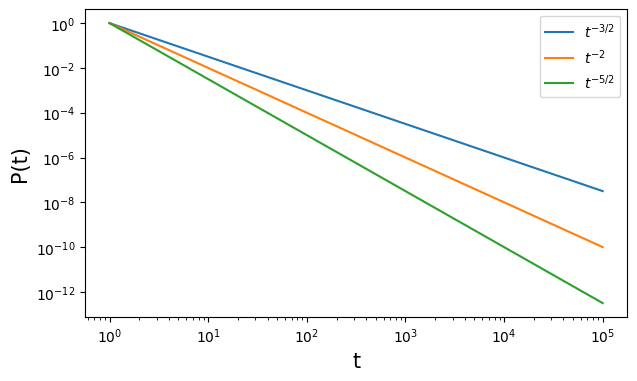
\includegraphics[width= 0.6\textwidth]{ley de potencias.png}
\caption{Representation of a power-law distribution. The slope of the double logarithm plot is the exponent of the distribution.}
\label{f:ley de pot}
\end{figure}

The classical toy model to describe criticality is the Ising model \cite{ising1925}, which describes the dependence on the temperature of the magnetic properties of metals. The Ising model 
shows a phase transition at a critical temperature $T_c$, separating
an ordered phase where the magnet's spins are aligned and when the temperature is lower than the critical temperature, and a disordered phase,
dominated by thermal fluctuations when $T>T_c$. Ising model is an example of criticality in a system in equilibrium, but these phenomena are also present in systems out of equilibrium. 
Some of the most studied systems in this context are contact processes due to their simplicity which are used to study activity propagation in a network.
The contact processes dynamics are based on the state of the system's constituents, which can be active or inactive, and they can change their state by interacting which 
each other at a certain rate. For instance, an active site can activate
an inactive site with a rate $\lambda$ which will be our control parameter and the inactive site can deactivate with a rate $\mu$. 
These rates will be the key to understanding the system's behaviour. In order to analyze the macroscopic properties of the system, we need to define the order parameter, 
which is a quantity that allows us to establish the phase \cite{wilting201925}. An example is shown in Figure \ref{f:order_parameter}.

\begin{figure}[H]
    \centering
    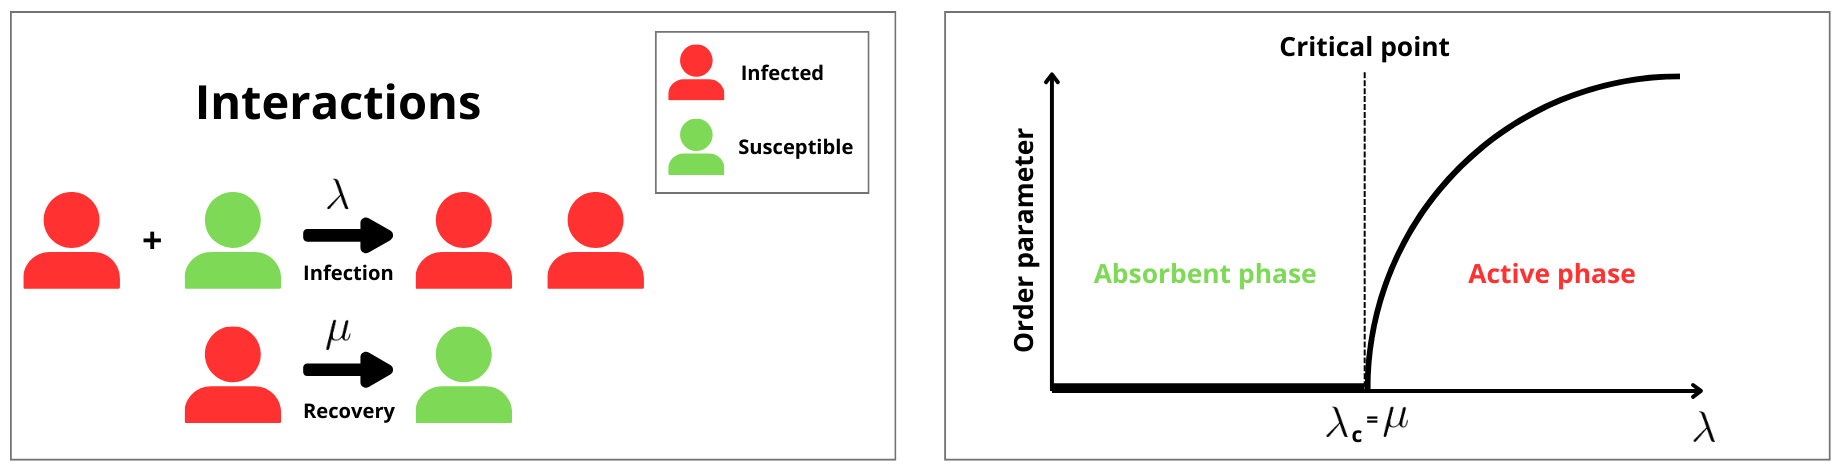
\includegraphics[width=0.95\textwidth]{phase transition.png}
    \caption{On the left, the dynamics of the SIS (Susceptible-Infected-Susceptible) model, which is a typical contact process for disease spreading \cite{pastor2015epidemic}. 
    On the right, the order parameter versus 
    the control parameter; in this case, the control parameter would be the infection rate $\lambda$. The order parameter is the fraction of infected individuals. 
    The SIS model has a critical point (in a fully-connected network) at $\lambda=\lambda_c=\mu$.}
    \label{f:order_parameter}
\end{figure}

Two other classic examples that are related to the results of this work are (critical) branching processes \cite{harris1963theory} and percolation processes \cite{stauffer2018introduction}. 
The first one is used for example to model phenomena 
related to offspring. In a simplified way we can say that a parent can have a random number of children given by a probability distribution with a mean value of $n$. We can discern between
subcritical, critical and supercritical branching processes depending on this value. For the subcritical case, $n<1$, and the process will die out eventually because the number of children
will decrease on average with each generation. For the supercritical case, $n>1$, the descendant population will grow exponentially. The most interesting situation is the critical case, $n=1$, 
where we will have, in average, power law distributions for the tree size (number of descendants) and the tree depth (number of generations) with exponents $\alpha\sim Z=3/2$ and $\tau\sim D=2$ respectively 
\cite{notarmuzi2021percolation}. A representation of these situations is shown in Figure \ref{f:branching_processes}.

\begin{figure}[H]
    \centering
    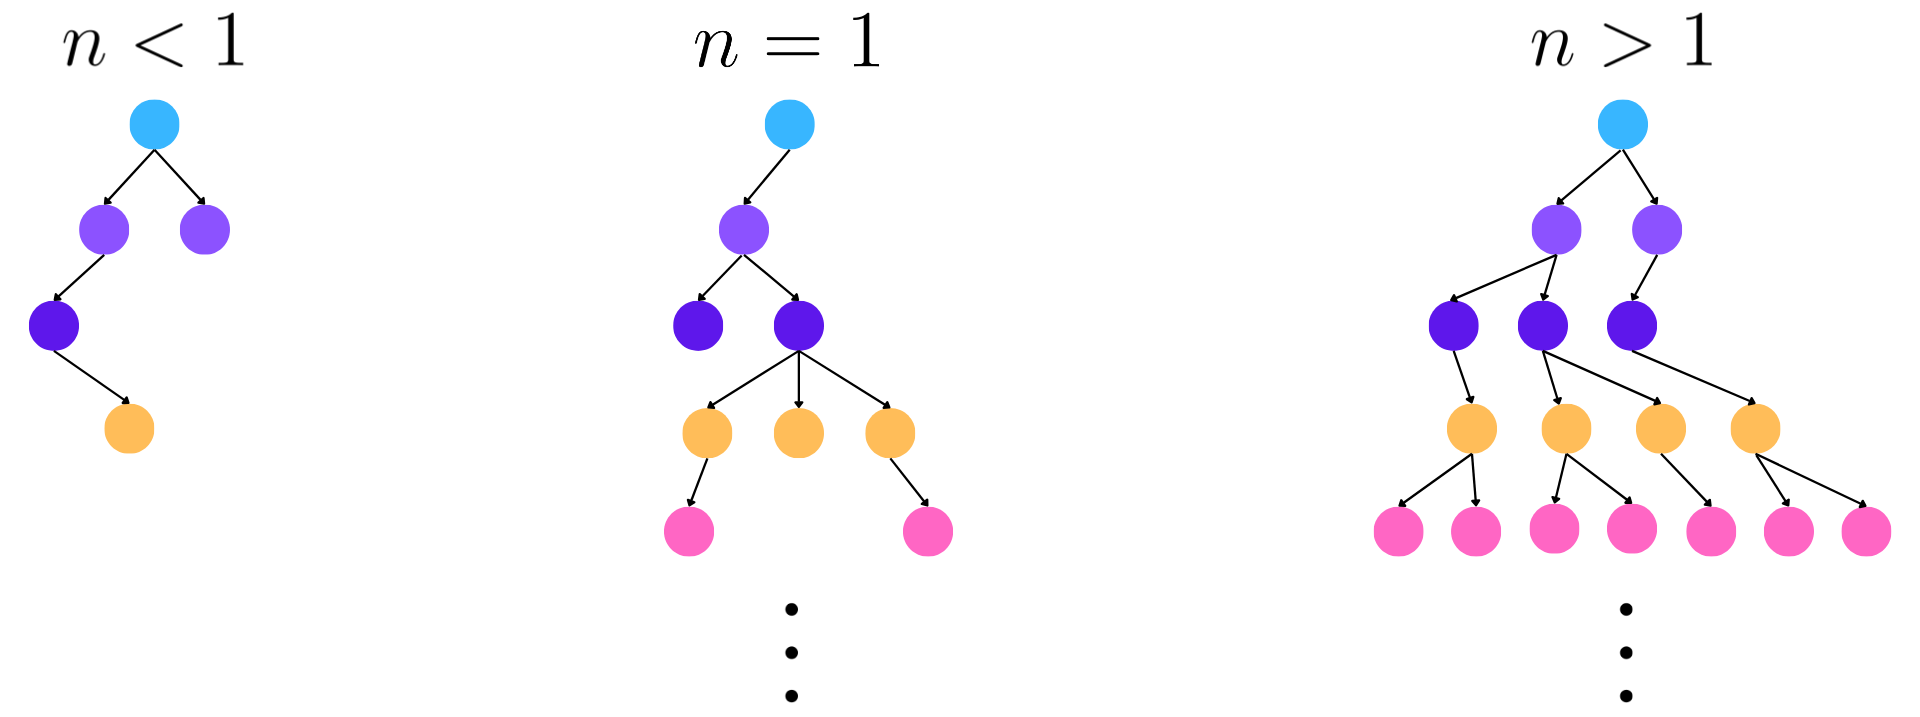
\includegraphics[width=0.7\textwidth]{Branching processes.png}
    \caption{On the left, a subcritical branching process, in the middle, a critical branching process and on the right, a supercritical branching process. Each color represents a different
    generation.}
    \label{f:branching_processes}   
\end{figure}

As a last example, we present percolation. These processes are generally used to model the flow of a fluid through a porous medium. Taking into account that this master 
thesis is related to living systems, there is no better example that relates the model with the topic, and physics (indeed, physicist) than an Italian coffee maker. Here, the porous 
medium is coffee, and the fluid is water. To describe the percolation process in a simple way, we can say that coffee makes a square lattice, and the water will flow through the nodes 
with a certain probability $p$, which depends on the pressure exerted during the pressing process. 
We can define clusters of connected nodes (in this situation, we are only interested on the vertical connections in order to make coffee)
for a given probability, and we also define the order parameter as the size of the largest cluster. 
Same as with branching processes, we can discern between subcritical, critical and supercritical percolation processes depending on the value of $p$. For the subcritical case, $p<p_c$,
the largest cluster will be smaller than the system size, describing a situation in which the water is not able to flow through the coffee. Conversely, in the supercritical case, $p>p_c$,
a lot of cluster will be of the size of the system, describing a situation in which the water flows through the coffee very easily, getting a watery coffee. 
In the same manner as the branching processes, the most interesting situation is the critical case, $p=p_c$. The critical point describes a situation in which the water can flow through the
coffee, but not extremely easily (as would happen in the supercritical case, $p>p_c$) and therefore extracts the coffee aroma in an optimal way. In the critical case, the cluster size, which 
is the number of clusters given a volume, $s$, normalized by the total volume, follows a power law distribution $n_s\sim s^{-\tau}$.
A representation of these situations is shown in Figure \ref{f:percolation}.

\begin{figure}[H]
    \centering
    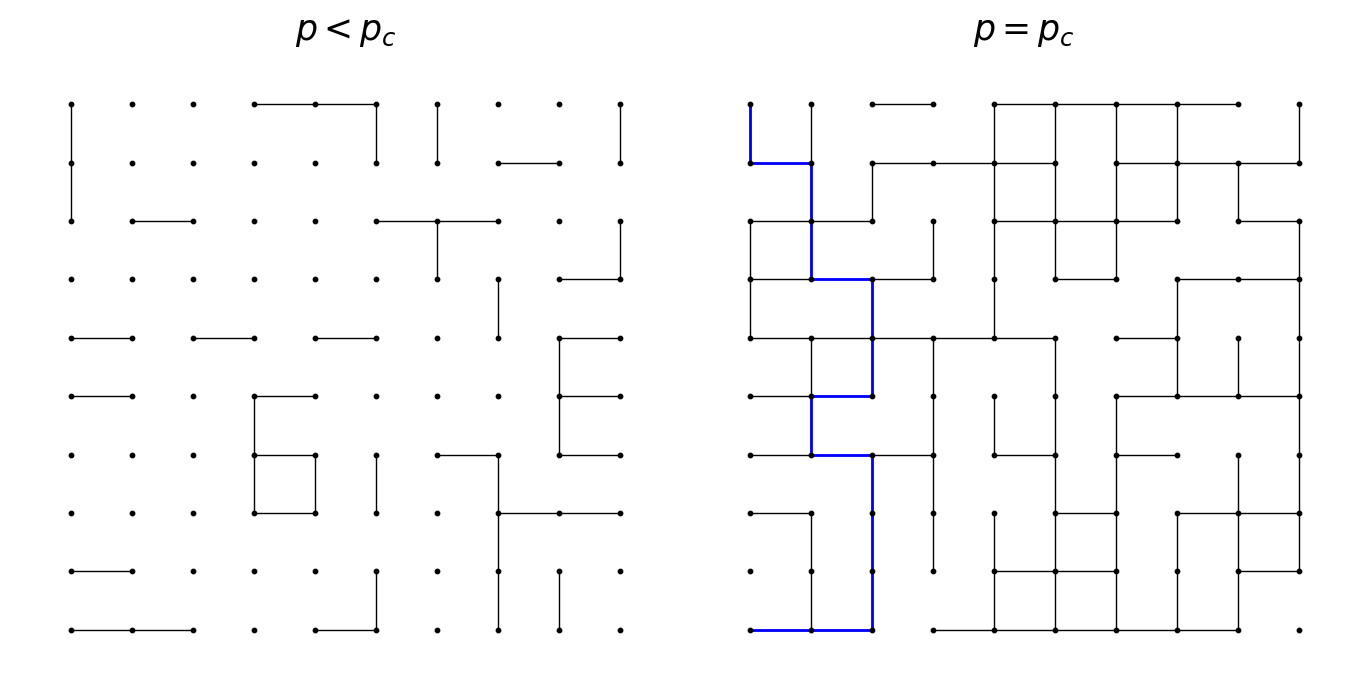
\includegraphics[width=0.9\textwidth]{percolacion.png}
    \caption{On the left, a subcritical percolation process; on the right, a critical percolation process. The blue line represents a percolant cluster.}
    \label{f:percolation}
\end{figure}
For our purposes, we will be interested in 1D percolation, whose exponents are $\alpha=2$ for the cluster size and $\tau=2$ for the duration \cite{stauffer2018introduction}. 
Having seen these examples, we move on to a brief introduction to point processes, which will lead us to another context to discuss criticality.

\section{Point processes} \label{sec:point_processes}
Within the large framework of complex systems, stochastic processes lend us a hand to decypher properties of living systems, bridging randomness with structured behaviour.
These processes are used to model the dynamics of systems that evolve randomly over time. This is why they are ideal for describing natural phenomena such as 
the spread of diseases \cite{Chowell}, social networks \cite{castellano2009statistical} or ecological systems \cite{azaele2016statistical}. Mathematically, a stochastic process
is a collection of random variables \cite{McKane}, generally ordered in time $ \{X_t\}_{t \in T} $, where $t$ is the time and $X_t$ is the system state at time $t$. $T$ is the time index set, 
which can be discrete or continuous. In this work we will focus on the continuous case because we are interested in the study of point (Hawkes) processes for modeling neurons. 

Point processes are a type of stochastic process that describes the occurrence of events in time or space. We will be interested in time point processes because 
we are going to model the spiking activity of neurons. For our purposes, they will be characterized by two parameters, the time of occurrence
of the events $t_k$ and the intensity or rate of occurrence of these events $\lambda(t)$. This rate tells us how likely it is that an event occurs at time $t$ given the history of the process, 
as pictured in Figure \ref{f:point_process}.

\begin{figure}[H]
    \centering
    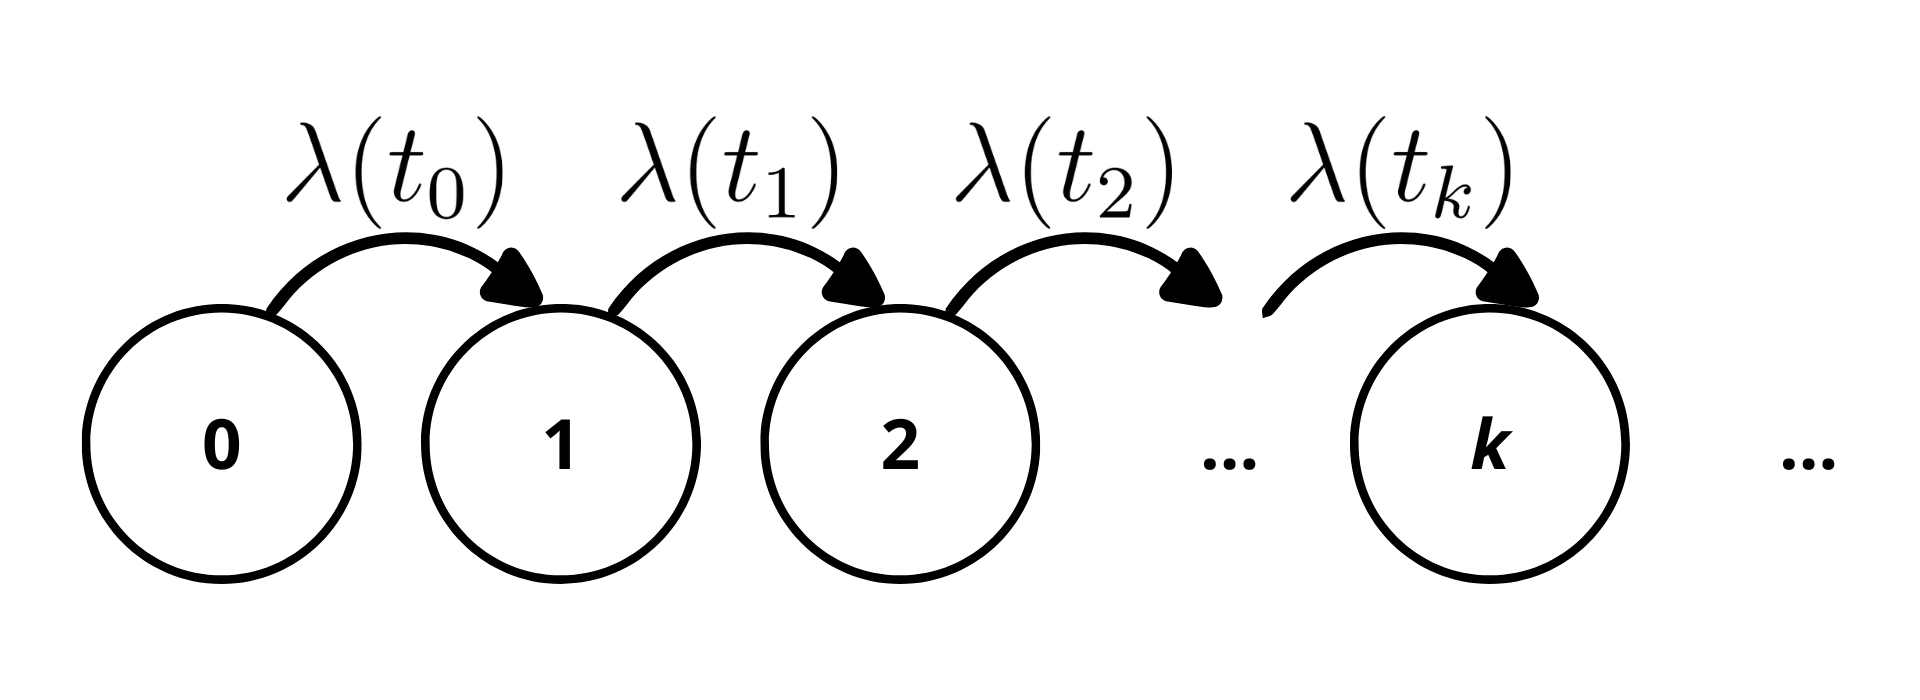
\includegraphics[width=0.85\textwidth]{Point process.png}
    \caption{Representation of a point process. The intensity function $\lambda(t)$ is a time-dependent function which represents the rate of occurrence of an event.}
    \label{f:point_process}
\end{figure}

\subsection{Poisson processes} \label{subsec:Poisson_processes}

In the more general case, the rate is a function of the history of the process, which makes the process non-Markovian, but in our case, it will be a Markovian process, which means that the rate 
depends only on the last event that occurred, as we will see. An example of a Markovian point process is the Poisson process, which is simple and one of the most studied point processes because 
it describes events that occur independtly in time, such as the arrival of customers at a store or occurrence of defects on a production line. They are also present in some physics phenomena,
for instance, the decay of radioactive particles or the arrival of photons at a detector. These processes are characterized by the rate of occurrence of events $\lambda$, 
which is independent of the state of the system.
The dynamics of these processes are described by the Poisson distribution, which is the probability distribution that the random variable $N$ takes the value $n$ and describes the 
probability that $n$ events occur in a given time interval is:

\begin{equation}
    P(N=n) = \dfrac{\lambda^n}{n!}e^{-\lambda}.
    \label{eq: Probabilidad proceso de Poisson homogéneo}
\end{equation}
Furthermore, the mean value and the variance of the distribution are equal to $\lambda$. Poisson processes can be homogeneous or inhomogeneous, depending on whether the rate is constant
or time-dependent. In Figure \ref{f:poisson} we can see an example of a homogeneous Poisson process.

\begin{figure}[H]
    \centering
    \includegraphics[width=0.95\textwidth]{Poisson probabilidad y nº eventos.png}
    \caption{Left: event number in time for different rates. Right: probability of having a certain number of events for different rates.}
    \label{f:poisson}
\end{figure}

\subsection{Hawkes processes} \label{subsec:Hawkes_processes}

On the other hand, if we consider a non-homogeneous Poisson process, the rate is a function of time, $\lambda(t)$. One example of inhomogeneous Poisson processes is in the Hawkes processes, which 
describes a process that is self-exciting, i.e. the more events happen in a given time window, the more events are likely to happen in the next time window.
The rate can be written in several ways \cite{notarmuzi2021percolation,kanazawa2021ubiquitous,dassios2013exact,laub2021elements}. We will use the expression from \cite{notarmuzi2021percolation}:

\begin{equation}
    \lambda(t|t_1, \ldots, t_k) = \mu + n\sum_{i=1}^k \phi (t-t_i),
    \label{eq: Hawkes rate}
\end{equation}

where $\mu$ is the background rate of a homogeneous Poisson process, $n$ is a parameter that controls the strength of the self-excitation, and $\phi(t)$ is the kernel function that
describes the influence of past events on the future rate. The kernel function must be a non-negative and non- monotonically-increasing function that integrates to 1.
Typical choices for the kernel function are the exponential or power-law functions, in this work, we will focus on the exponential kernel. 
Eq. \ref{eq: Hawkes rate} models a firing rate that increases by a quantity $n$ with each event, and recovers (guided by the kernel function) toward $\mu$ in the absence of any events 
(see Figue \ref{f: Hawkes rate}).
We can see that the rate depends on the history of the process, making it non-Markovian in general, but with an exponential kernel, the dependence on the 
past events decays exponentially fast. In fact, it can be shown that the process becomes Markovian, see Appendix \ref{ch:Anexo calculos}.

Despite being a Markovian process, it is still an inhomogeneous Poisson process because the rate is not constant. In addition, it is a self-exciting process, which means that the occurrence
of an event increases the probability of the occurrence of another event. This is why it is used to model the spiking activity of neurons, where the occurrence of a spike increases the
probability of the occurrence of another spike \cite{munoz2018colloquium}. 
This self-excitation will enable the appearance of bursts of activity that we will measure. The parameters chosen for the kernel function 
will be $\alpha=\beta=1$ and we will vary the background rate $\mu$ from values much smaller than 1 to values greater than 1. In Figures \ref{f: Hawkes rate} and \ref{f: Hawkes rate 2}
we can see typical diagrams of Hawkes processes with these parameters. Details on the numerical simulation are explained later on, in Chapter \ref{ch:metodologia}.

\begin{figure}[H]
    \centering
    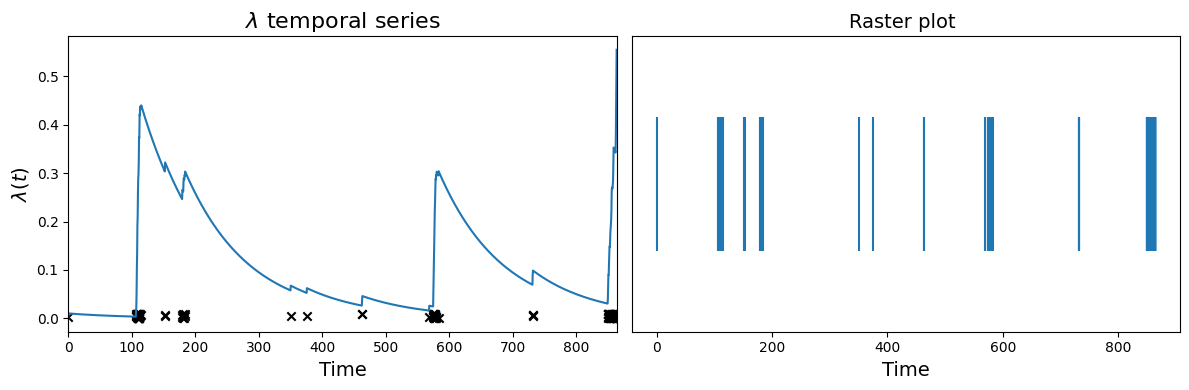
\includegraphics[width=0.95\textwidth]{Hawkes mu 0.01.png}
    \caption{On the left, a temporal series of $K=150$ events of a Hawkes process with $\mu=0.01$, on the right, a raster plot of the same process.}
    \label{f: Hawkes rate}
\end{figure}

\begin{figure}[H]
    \centering
    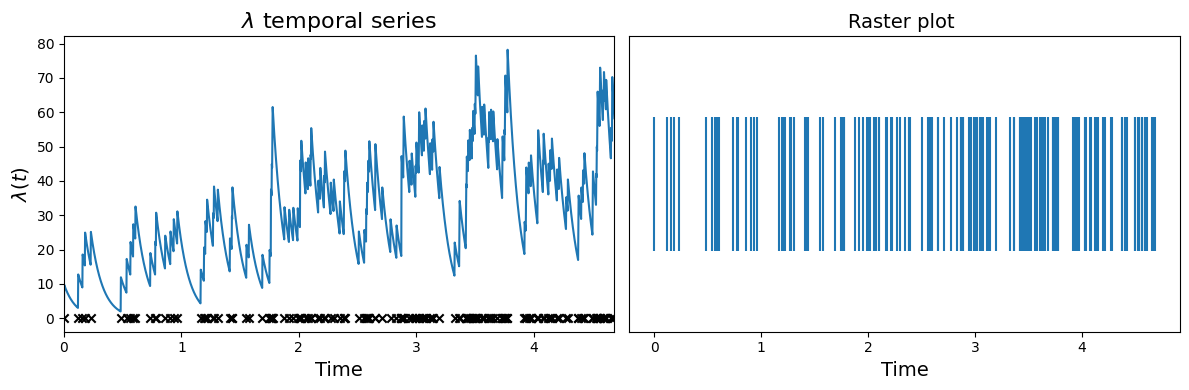
\includegraphics[width=0.95\textwidth]{Hawkes mu 10.png}
    \caption{On the left, a temporal series of $K=150$ events of a Hawkes process with $\mu=10$, on the right, a raster plot of the same process.}
    \label{f: Hawkes rate 2}
\end{figure}

As shown in Figure \ref{f: Hawkes rate}, when the background rate is smaller than 1, events are less likely to occur, but when they do, they tend to form avalanches of activity thanks 
to the self-excitation. On the other hand, when the background rate is greater than 1, events occur more frequently, forming avalanches of activity more frequently and longer, as
shown in Figure \ref{f: Hawkes rate 2}. If we ignore the time of occurrence of the events and focus only on the structure of $\lambda$ and therefore of the events, we can see that
the process with $\mu=0.01$ has a bursty structure, while the process with $\mu=10$ has a more regular structure. This phenomenon is exposed in Figures \ref{f: Hawkes rate burst} and
\ref{f: Hawkes rate burst 2}.

\begin{figure}[H]
    \centering
    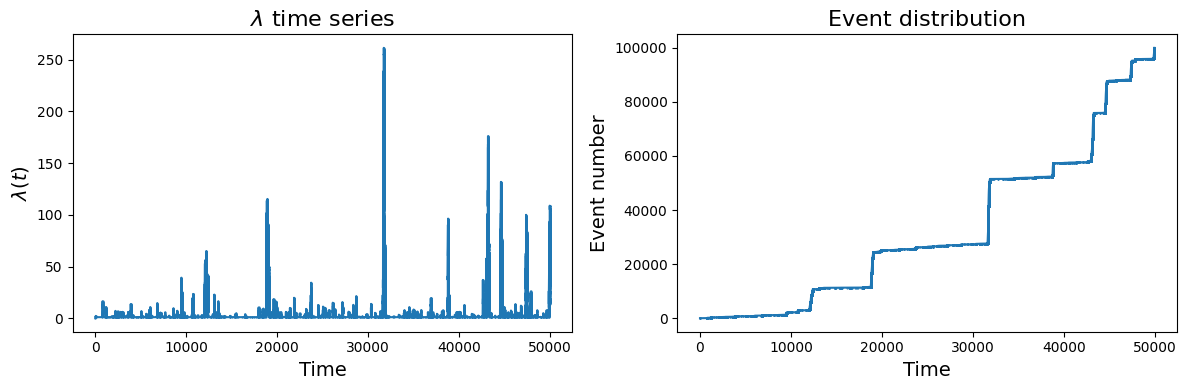
\includegraphics[width=0.95\textwidth]{Hawkes mu 0.01 events.png}
    \caption{First, a temporal series of $K=10^5$ events of a Hawkes process with $\mu=0.01$, on the right, the event distribution. Thicker blue bars represent avalanches of activity.}
    \label{f: Hawkes rate burst}    
\end{figure}

\begin{figure}[H]
    \centering
    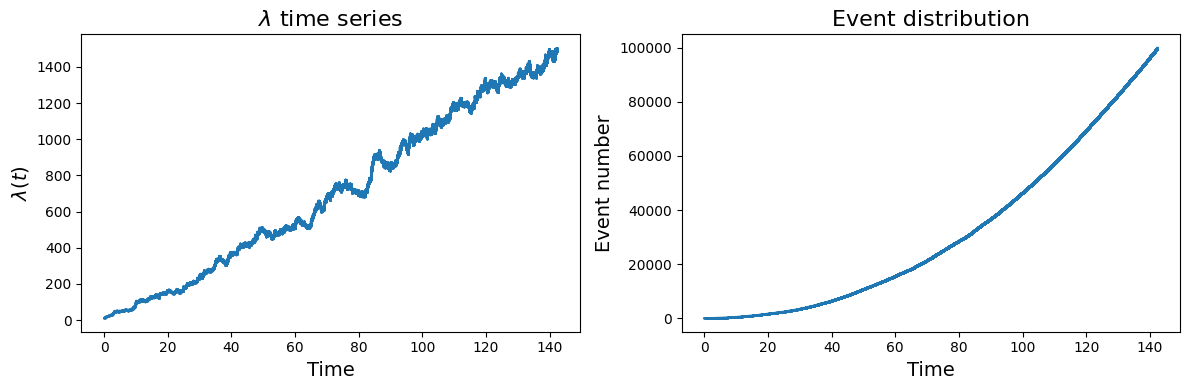
\includegraphics[width=0.95\textwidth]{Hawkes mu 10 events.png}
    \caption{First, a temporal series of $K=10^5$ events of a Hawkes process with $\mu=10$, on the right, the event distribution.}
    \label{f: Hawkes rate burst 2}    
\end{figure}

In most cases, the motivation for studying point processes is counting the events, but in our case, we are also interested in the time of occurrence of the events
which will let us define bursts or avalanches of activity that we will use to describe the dynamics of the system. 
As we have said previously, $\alpha = 1$, $\beta = 1$, making $n$ the parameter that controls the strength of the self-excitation. Essentially, $n$ and $\alpha$ play the same role,
so we will use them indistinctly. The previous figures showed the dynamics for $n=1$, making the system critical as a critical branching process \cite{notarmuzi2021percolation}, 
such the one that we previously described. We will also study the dynamics for $n=2$ and two coupled Hawkes processes.


\subsubsection{Bivariate Hawkes processes} \label{subsubsec:Coupled_Hawkes_processes}
With the previous knowledge, we can model an isolated neuron working in different regimes, but as we know, the brain is composed of an enormous number of neurons connected to each 
other, forming a network. Moreover, neurons can be classified into two kinds, excitatory and inhibitory neurons. To get closer to modeling the brain, we will also generate two coupled
Hawkes processes, one corresponding to an excitatory population and the other to an inhibitory population, or just an excitatory and inhibitory neuron. 
Both populations (neurons) will have a background rate  $\mu_E$ and $\mu_I$, and they will be able to interact with each other and with themselves, the ``strength'' of the interactions 
will be controlled by the parameters $n_{EE}$, $n_{EI}$, $n_{IE}$ and $n_{II}$. In most cases, the auto-inhibition can be considered negligible. 
These interactions are illustrated in Figure \ref{f: Hawkes coupled} and the equations to model the interaction in Eq. \ref{eq: ecuaciones bivariate}.

\begin{equation}
    \begin{split}
        \lambda_E =& \mu_E + n_{EE}\sum_{i=1}^{k}\phi(t-t_i) + n_{EI}\sum_{i=1}^{k}\phi(t-t_i)\\
        \lambda_I =& \mu_I + n_{IE}\sum_{i=1}^{k}\phi(t-t_i) + n_{II}\sum_{i=1}^{k}\phi(t-t_i)
    \end{split}
    \label{eq: ecuaciones bivariate}
\end{equation}

\begin{figure}[H]
\centering
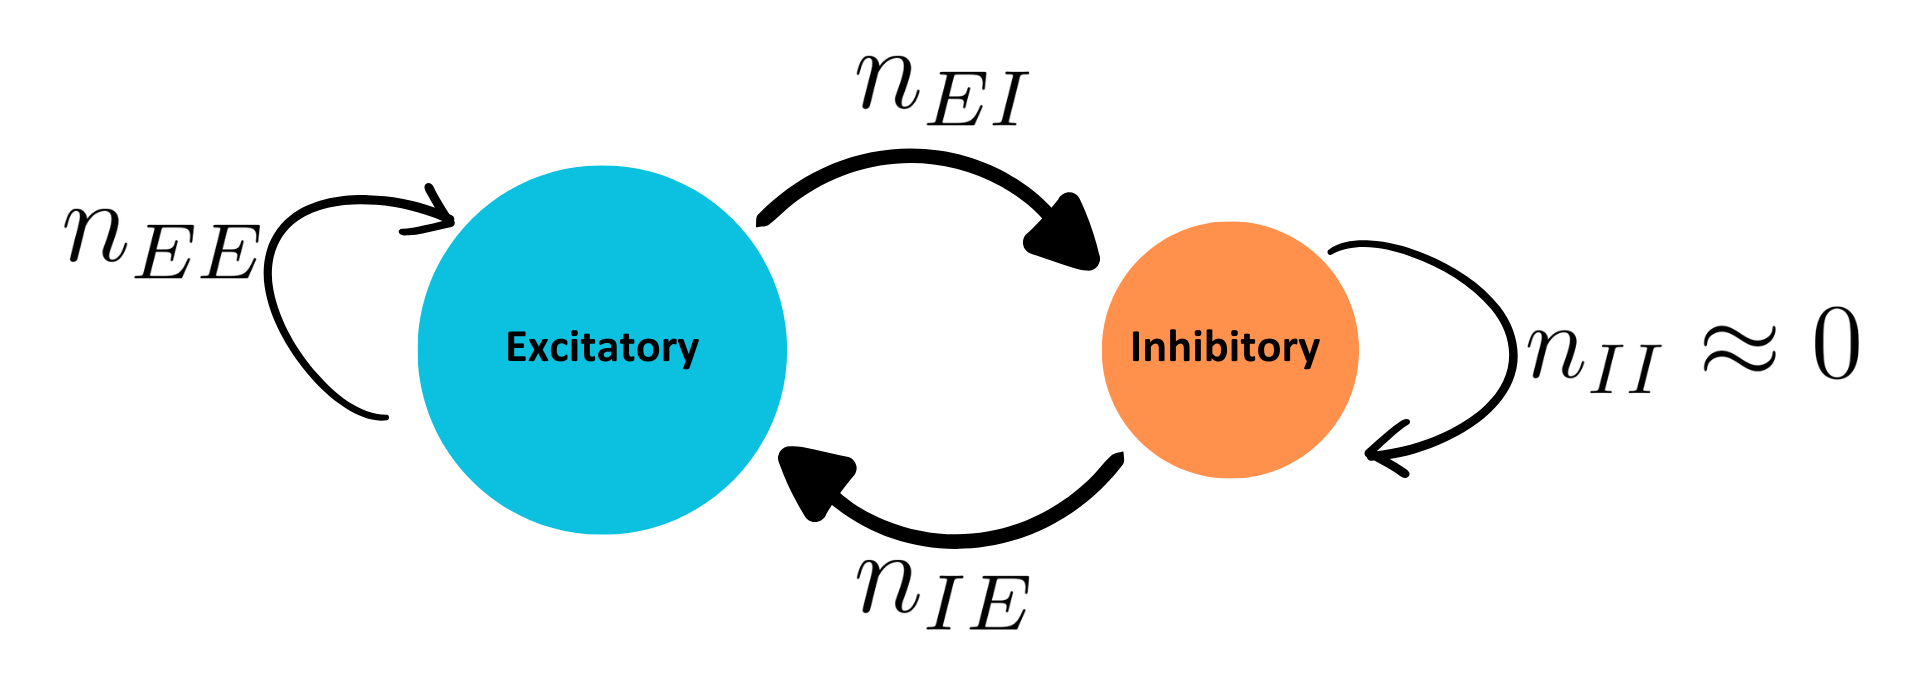
\includegraphics[width=0.7\textwidth]{Esquema inhibición-excitación.png}
\caption{Scheme of the interaction between the excitatory and inhibitory populations. As illustrated, the excitatory population can excite itself and the inhibitory population, while the
inhibitory population can only inhibit the excitatory population, because on most cases the auto-inhibition is negligible \cite{kalle2018growing}.}
\label{f: Hawkes coupled}
\end{figure}
